\chapter{Metodologia}
O desenvolvimento do ESC será realizado seguindo uma abordagem de engenharia de sistemas, partindo da especificação da carga e fonte de energia, passando pelo dimensionamento dos estágios de potência e controle, e finalizando com a validação experimental. A metodologia está estruturada em: definição da arquitetura do sistema, dimensionamento do hardware de potência, desenvolvimento do firmware de controle, simulação computacional e, por fim, a montagem e prototipagem do dispositivo.

\section{Arquitetura do Sistema}
Para a elaboração do projeto físico é necessário o levantamento dos requisitos mínimos que o projeto deve atender, como a categoria de motores e sua fonte de alimentação. A arquitetura proposta consiste em um fluxo de energia que parte de uma bateria de alta descarga, passa por um inversor trifásico controlado, o ESC, e alimenta o motor BLDC. O controle é supervisionado por um microcontrolador que monitora os parâmetros e gera os sinais de modulação.

O projeto do circuito começa pelo levantamento das especificações de carga, seguido pelo dimensionamento da fonte de energia e dos semicondutores de potência. Em paralelo, projeta-se o sistema de controle, definindo o microcontrolador adequado, a lógica de acionamento dos drivers de gate e as estratégias de proteção térmica e de sobrecorrente.

\section{Dimensionamento e Hardware de Potência}
A escolha dos componentes de potência baseia-se nas especificações do motor selecionado, garantindo margens de segurança para operação em regime contínuo e transitório.

\subsection{Especificações do Motor e Carga}
O motor BLDC Turnigy XK3674-$2200KV$ é um modelo comercial projetado principalmente para Automodelismo, sendo do tipo Inrunner possui quatro polos, $2200KV$, Tensão Nominal de $25,2V$, Corrente Nominal de $70A$ e sendo capaz de produzir até $1750W$ de potência. A velocidade e torque a vazio do motor, como já vistos nos segmentos anteriores, é de $55440 RPM$ e $0,3 Nm$, desconsiderando efeitos dissipativos, como o atrito.

\begin{figure}[h]
    \centering
    \caption{Motor Brushless Turnigy XK3674-$2200KV$.}
    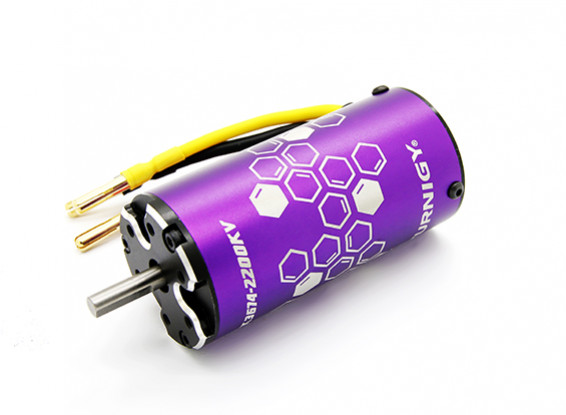
\includegraphics[width=8cm]{imagens/Turnigy XK3674-2200KV.jpg}
    \caption*{Fonte:\cite{turnigyMotor}.}
 \label{Motor Brushless Turnigy XK3674-2200KV}
\end{figure}

\subsection{Fonte de Alimentação Principal (Bateria)}
Em uma aplicação móvel para o ESC devemos fazer uso de baterias como a única fonte de potência para alimentar todo o sistema. Os valores nominais de tensão e corrente do motor a devem ser supridos pela bateria, por volta de $26V$ e $70A$, mas considerando momentos de pico de corrente como por exemplo, uma situação de rotor travado ou de inversão de sentido de rotação é usada uma margem de segurança arbitrária de $30\%$, logo a bateria deve ser capaz de entregar $91A$ de corrente na descarga, um valor considerado alto para baterias.

Atualmente, a tecnologia de bateria com a maior taxa de descarga disponível comercialmente é a bateria de lítio de polímero (LiPo), podendo atingir taxas de descarga muito altas, que podem ultrapassar a $100C$, dependendo da aplicação e do design. 

Baterias LiPo tem três principais características:
\begin{itemize}
\item Configuração das Células (S): A nomenclatura "S" (do inglês \textit{Series}) indica o número de células de polímero de lítio conectadas eletricamente em série no interior do \textit{pack}. Nesta configuração, a tensão de cada célula se soma enquanto a capacidade de corrente se mantém.
    Considerando a tensão nominal de uma célula LiPo como $3,7V$ e a tensão de carga máxima como $4,2V$, a tensão total do \textit{pack} ($V_{\text{pack}}$) é dada por:
    \begin{equation}
        V_{\text{pack}} = N_S \cdot V_{\text{célula}}
    \end{equation}
    Assim, a bateria $6S$ especificada para este projeto possui 6 células, resultando em uma tensão nominal de $22,2V$ e uma tensão máxima de $25,2V$ (plenamente carregada). Este parâmetro é crítico para o dimensionamento do $K_V$ do motor e da tensão máxima dos MOSFETs; 
\item Capacidade: Indica a quantidade de carga que a bateria pode fornecer antes de ser descarregada completamente, Normalmente é medida em miliampere-horas ($mAh$) ou ampere-horas ($Ah$);
\item Taxa de Descarga (ou \textit{C-rate}): Define a quantidade de corrente que a bateria pode fornecer sem danificar-se, é expressa em múltiplos de $C$.
\end{itemize}

Para calcular a corrente que tais baterias conseguem fornecer podemos aplicar a equação \ref{Corrente de uma bateria LiPo}, desconsiderando efeitos dissipativos ou a variação de tensão nominal que varia de acordo com o nível de carga da bateria, vale ressaltar que a capacidade da bateria deve estar em $Ah$.

\begin{equation}
I = C-rate \cdot Capacidade
\label{Corrente de uma bateria LiPo}
\end{equation}


Uma bateria comercial que atende as especificações do projeto é o modelo Turnigy Graphene Panther $1300mAh$ $6S$ $75C$, capaz de fornecer por volta de $97,5A$, superior a margem de segurança estabelecida. Vale ressaltar que a baterias entrega de tensão nominal $22,2V$, inferior a tensão nominal o que para motores BLDC não é um problema, resultando apenas na redução da  sua velocidade nominal de $55440 RPM$ para $48840RPM$ a vazio, uma redução de aproximadamente $12\%$. 

\begin{figure}[h]
    \centering
    \caption{Turnigy Graphene Panther $1300mAh$ $6S$ $75C$.}
    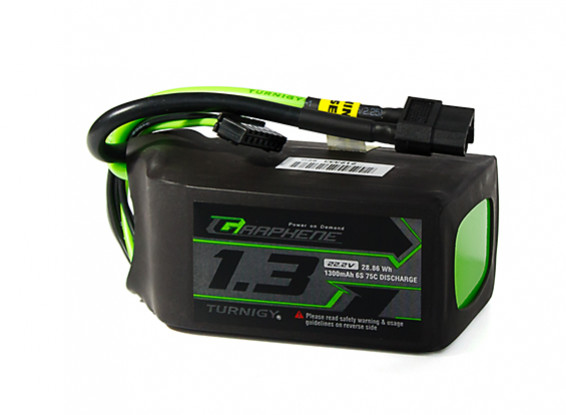
\includegraphics[width=9cm]{imagens/Turnigy Graphene Panther 1300mAh 6S 75C.jpg}
    \caption*{Fonte:\cite{turnigyBattery}.}
 \label{Turnigy Graphene Panther 1300mAh 6S 75C}
\end{figure}

\subsection{Sistema de Proteção Contra Sobrecorrentes}

Dada a baixa resistência interna das baterias de Lítio-Polímero (LiPo) e a alta capacidade de corrente do sistema ($>90 \text{ A}$), um eventual curto-circuito no estágio de potência resultaria em correntes de falha de magnitude catastrófica, com risco real de incêndio e explosão da fonte de energia.

Para mitigar este risco, projetou-se um sistema de proteção passiva composto por um fusível do tipo \textbf{MIDI} de $100 A$, instalado em série com o cabo positivo da bateria, externo à placa de circuito impresso (PCB). Esta topologia foi escolhida baseada em dois critérios:

\begin{itemize}
    \item \textbf{Tipo de Fusível (MIDI):} Diferente dos fusíveis de lâmina automotivos comuns (ATO/ATC), o padrão MIDI possui terminais para fixação por parafusos (M5 ou M6). Isso garante uma pressão de contato elevada, minimizando a resistência de contato ($R_{contato}$) e, consequentemente, o aquecimento indesejado no ponto de conexão sob altas correntes.
    
    \item \textbf{Instalação Externa (Off-Board):} A alocação do fusível no cabo, ao invés da PCB, preserva a integridade das trilhas de cobre em caso de fusão violenta do elemento condutor. Além disso, facilita a manutenção em campo e remove uma fonte de calor concentrada de perto dos transistores de potência.
\end{itemize}

O dimensionamento de $100 A$ oferece uma margem de segurança de aproximadamente $10\%$ sobre a corrente de pico estimada do motor ($90 A$), garantindo que o dispositivo atue apenas em casos de falha real (curto-circuito ou travamento mecânico do rotor), sem interrupções espúrias durante a operação nominal.

\subsection{Filtragem do Barramento DC (Link DC)}

Considerando a bateria LiPo como fonte primária de energia, e sabendo que a indutância dos cabos de alimentação pode gerar transientes destrutivos, projetou-se um estágio de filtragem para o barramento DC.

O dimensionamento dos capacitores do \textit{Link DC} priorizou a minimização da Resistência Série Equivalente (ESR) para evitar o superaquecimento causado pela corrente de ripple. A capacitância mínima ($C_{bus}$) foi estipulada seguindo a regra prática de engenharia para ESCs de alta performance, que recomenda aproximadamente $220\mu F$ para cada $20A$ de corrente de fase:

\begin{equation}
    C_{bus} \approx \frac{I_{peak}}{20} \cdot 220\mu F = \frac{90}{20} \cdot 220\mu F \approx 990 \mu F
\end{equation}

Dessa forma, a topologia final do barramento de entrada é composta por:
\begin{itemize}
    \item Conector de alta corrente XT90 (anti-centelha) para conexão com a bateria;
    \item Dois capacitores eletrolíticos \textit{Low-ESR} de \textbf{$470\mu F$ / $35V$} ligados em paralelo (Total: $940\mu F$), posicionados o mais próximo possível dos drenos dos MOSFETs de alta para minimizar o loop de indutância.
\end{itemize}

Esta escolha assegura que o banco de capacitores suporte a corrente $I_{RMS}$ estimada do inversor, mantendo a temperatura de operação dentro dos limites seguros especificados para a série \textit{Low-ESR}.

\subsection{Dimensionamento do Inversor (MOSFETs)}
Para o estágio de comutação da ponte inversora trifásica, a escolha do MOSFET foi governada por dois parâmetros críticos: a tensão de ruptura dreno-fonte ($V_{DSS}$), representa o limite máximo de tensão que o dispositivo suporta em seus terminais principais enquanto está em estado de não-condução e a capacidade de dissipação térmica. Considerando que a bateria 6S carregada atinge $25,2V$, e prevendo picos de tensão indutiva ($V_{spike}$) durante o chaveamento, selecionou-se o modelo \textbf{IRFS7530TRL7PP}. Este componente possui um $V_{DSS}$ de $60V$, oferecendo uma margem de segurança superior a 100\% em relação à tensão do barramento DC.

A validação térmica foi realizada considerando a resistência em condução ($R_{DS(on)}$) máxima do componente, que é de aproximadamente $1,4 m\Omega$. Para a corrente de pico projetada de $91A$, a potência dissipada estimada ($P_{diss}$) é dada por:

\begin{equation}
    P_{diss} = I^2 \cdot R_{DS(on)} = 91^2 \cdot 0,0014 \approx 11,6 W
\end{equation}

Embora o encapsulamento D2PAK-7 suporte altas correntes, a dissipação de aproximadamente $11,6W$ exige o uso de uma área de cobre estendida na PCB ou acoplamento com dissipador térmico externo para manter a temperatura de junção dentro dos limites operacionais seguros.



\subsection{Driver de Gate e Circuito de Bootstrap}
O microcontroladores no geral operam com lógica de $3,3V$ ou $5V$, tensão insuficiente para saturar o gate dos MOSFETs de potência, que requerem tipicamente entre $10V$ e $15V$ para garantir a mínima resistência $R_{DS(on)}$. Além disso, o acionamento dos MOSFETs do lado alto (\textit{High-Side}) exige uma tensão flutuante superior à tensão da bateria.

Para solucionar essa interface, foi selecionado o driver de meia-ponte \textbf{IR2110}, capaz de fornecer correntes de pico de até $2A$ para carga e descarga rápida da capacitância de gate ($Q_g$). O driver é alimentado com $15V$ (derivados do circuito BEC), garantindo a saturação completa dos transistores.

De acordo com o datasheet do IRFS7530, a resistência interna de gate típica é de $2,1 \Omega$. Para limitar a corrente de source ($I_{source}$) ao máximo de $2A$ sob a tensão de alimentação de $15V$, a resistência total do caminho de gate deve ser:

\begin{equation}
    R_{total} \geq \frac{V_{drv}}{I_{max}} = \frac{15V}{2A} = 7,5 \Omega
\end{equation}

Subtraindo a resistência interna do componente, obtém-se o valor mínimo teórico para o resistor externo:

\begin{equation}
    R_{g,ext} = R_{total} - R_{G,int} = 7,5 \Omega - 2,1 \Omega = 5,4 \Omega
\end{equation}

Para assegurar uma margem de segurança e maior amortecimento, selecionou-se o valor comercial de \textbf{$10 \Omega$}. Com este valor, o tempo de comutação estimado ($t_{sw}$) para a carga total de gate ($Q_g \approx 360nC$) será:

\begin{equation}
    I_{med} \approx \frac{V_{drv}}{R_{g,ext} + R_{G,int}} = \frac{15V}{12,1 \Omega} \approx 1,24 A
\end{equation}

\begin{equation}
    t_{sw} \approx \frac{Q_g}{I_{med}} = \frac{360nC}{1,24A} \approx 290 ns
\end{equation}

Este tempo de transição de aproximadamente $290ns$ é adequado para a frequência de PWM do projeto (tipicamente $20kHz$ a $40kHz$), representando menos de $1,5\%$ do período total, o que garante baixas perdas por comutação sem comprometer a estabilidade eletromagnética.

Para o acionamento do \textit{High-Side}, utiliza-se a técnica de \textit{Bootstrap}. O capacitor de bootstrap ($C_{boot}$) foi dimensionado para sustentar a carga do gate durante o período de condução. Adotou-se o critério de projeto que recomenda que o capacitor seja capaz de armazenar uma carga pelo menos 15 vezes superior à carga total de gate ($Q_g$) do MOSFET \cite{adamsDT98}. Considerando o IRFS7530 com $Q_g \approx 360nC$:

\begin{equation}
    Q_{min} = 15 \cdot Q_g = 15 \cdot 360nC = 5,4 \mu C
\end{equation}

Para o banco de capacitores, optou-se por uma associação em paralelo de um capacitor eletrolítico de $10\mu F$ (reserva de energia) e um cerâmico de $100nF$ (para resposta em alta frequência). Alimentados pela tensão de $15V$ do driver, a carga total armazenada é:

\begin{equation}
    Q_{arm} = C_{boot} \cdot V_{drv} = 10\mu F \cdot 15V = 150 \mu C
\end{equation}

O valor obtido ($150 \mu C$) é significativamente superior ao mínimo requerido ($5,4 \mu C$), garantindo robustez. Além disso, a queda de tensão estimada no capacitor a cada ciclo de comutação ($\Delta V_{boot}$) é desprezível:

\begin{equation}
    \Delta V_{boot} = \frac{Q_g}{C_{boot}} = \frac{360nC}{10\mu F} = 0,036V
\end{equation}

Essa queda de apenas $36mV$ (0,24\% da tensão de alimentação) assegura que a tensão $V_{GS}$ aplicada ao MOSFET permaneça estável, garantindo a saturação completa do semicondutor.

\subsection{Determinação da Frequência de Chaveamento}

A definição da frequência de chaveamento ($f_{sw}$) é um parâmetro crítico no projeto de inversores de frequência de alta corrente, pois representa um \textit{trade-off} direto entre eficiência térmica, qualidade da forma de onda e conforto acústico. Para este projeto, optou-se pela frequência de \textbf{20 kHz}.

Esta escolha fundamenta-se em três critérios de engenharia principais e na validação de compatibilidade dos componentes selecionados:

\subsubsection{Análise de Perdas por Comutação}
As perdas de potência em um MOSFET durante a comutação ($P_{sw}$) são diretamente proporcionais à frequência de operação, conforme estabelecido na Equação \ref{eq:perdas} \cite{rashid2014power}:

\begin{equation} \label{eq:perdas}
P_{sw} = \frac{1}{2} V_{d} \cdot I_{o} \cdot (t_{on} + t_{off}) \cdot f_{sw}
\end{equation}

Onde $V_d$ é a tensão do barramento, $I_o$ a corrente de carga e $t_{on}/t_{off}$ os tempos de comutação.
O projeto utiliza transistores automotivos IRFS7530, que, embora robustos, apresentam uma carga total de gate ($Q_g$) significativa. A elevação da frequência para valores típicos de aeromodelismo (como $48 kHz$ ou $96 kHz$) resultaria em uma dissipação térmica excessiva nos semicondutores, exigindo sistemas de arrefecimento incompatíveis com o volume disponível. A frequência de $20 kHz$ mantém as perdas em um nível gerenciável pela dissipação passiva projetada.

\subsubsection{Mitigação de Ruído Acústico}
A operação de motores elétricos gera ruído audível devido à magnetostrição nas lâminas do estator e nas bobinas, excitadas pelos harmônicos da corrente PWM. Segundo Mohan, Undeland e Robbins (2003), recomenda-se que a frequência de chaveamento seja situada acima do limiar da audição humana.
Ao fixar $f_{sw}$ em $20 kHz$, o sistema opera na região ultrassônica, eliminando o zumbido agudo característico de inversores que operam em faixas inferiores (como $8 kHz$ ou $12 kHz$), garantindo conforto acústico na operação do veículo.

\subsubsection{Ripple de Corrente e Torque}
Para garantir um torque constante, a frequência de chaveamento deve ser suficientemente alta para interagir com a indutância do motor, limitando a ondulação de corrente (\textit{ripple}). Devido à ausência de dados de indutância e resistência no datasheet do fabricante (Turnigy), consideraram-se os valores típicos para motores BLDC de 4 polos (classe 3674) encontrados na literatura \cite{hanselman2003brushless}: indutância de fase na ordem de $L \approx 20 \mu H$ e resistência de $R \approx 10 m\Omega$.

Isso resulta em uma constante de tempo elétrica estimada de $\tau = L/R \approx 2 \text{ ms}$. Dado que o período de chaveamento a 20 kHz é de $T = 50 \mu s$, observa-se que $T \ll \tau$. Essa margem garante que a dinâmica elétrica do motor seja significativamente mais lenta que o chaveamento, assegurando a operação no modo de condução contínua com baixa ondulação de corrente \cite{hanselman2003brushless}.

\subsubsection{Validação da Compatibilidade do Driver}
Foi realizada a validação teórica do driver de gate IR2110 para assegurar sua operação estável na frequência definida. Segundo o datasheet do fabricante \cite{infineon2005}, o componente apresenta tempos de propagação típicos de $t_{on} = 120 \text{ ns}$ e $t_{off} = 94 \text{ ns}$. Considerando o período de $50 \mu s$, os atrasos do driver representam menos de $0,5\%$ do ciclo total, sendo desprezíveis para a dinâmica do controle.

Adicionalmente, calculou-se a corrente média de gate ($I_{g,avg}$) necessária para comutar os MOSFETs, considerando o pior caso de carga de gate ($Q_{g,max} = 354 \text{ nC}$) especificado no datasheet do IRFS7530 \cite{infineon7530}, conforme a Equação \ref{eq:igavg}:

\begin{equation} \label{eq:igavg}
I_{g,avg} = Q_{g,max} \cdot f_{sw} \approx 354 \text{ nC} \cdot 20 \text{ kHz} \approx 7,08 \text{ mA}
\end{equation}

O valor calculado de $7,08 mA$ está amplamente dentro da capacidade de dissipação térmica do IR2110 e situa-se muito abaixo do seu limite de corrente de pico ($2 A$), confirmando que o estágio de acionamento operará em regime seguro.

A frequência de $20 kHz$ foi validada teoricamente como o ponto ótimo de operação, equilibrando a minimização das perdas térmicas com a operação silenciosa e a integridade dos componentes de acionamento.

\subsection{Fonte de Alimentação Auxiliar}
Existem duas abordagens possíveis para a alimentação do microcontrolador e drivers: utilizar uma segunda bateria ou reduzir o nível de tensão da bateria principal. Para otimizar peso e volume, optou-se por um circuito BEC (\textit{Battery Elimination Circuit}).

Dentre as topologias disponíveis, destacam-se os conversores buck (step-down). O conversor Buck é amplamente utilizado para a redução de tensão, operando com elevada eficiência (tipicamente superior a $85\%$) \cite{TIBuckCalculation}. No projeto será aplicado o módulo comercial de baixo custo \textbf{LM2596}, um conversor buck de $150kHz$ e $3A$. O sistema é configurado em cascata: a tensão da bateria ($22,2V - 25,2V$) é regulada para $15V$ para alimentar os drivers IR2110, e subsequentemente reduzida para $5V/3,3V$ para o microcontrolador ESP32.

\begin{figure}[h] 
    \centering 
    \caption{Módulo Comercial LM2596.} 
    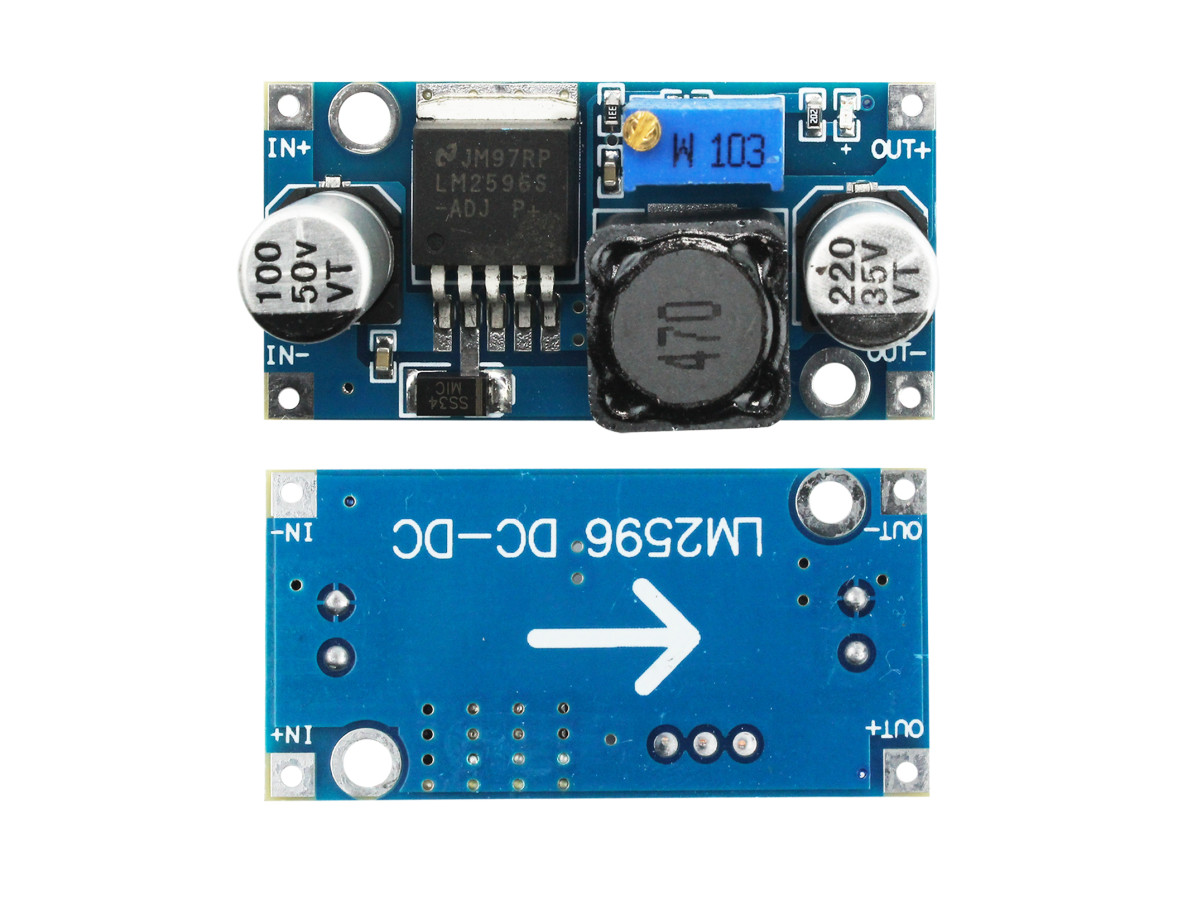
\includegraphics[width=7cm]{imagens/Módulo LM2596.jpg} 
    \caption*{Fonte:\cite{usinaInfoLM2596}.}
\end{figure}

\subsection{Sensoriamento de Corrente e Proteção (Shunt)}

Para implementar a proteção contra sobrecorrente e monitorar o consumo do sistema em tempo real, adotou-se a topologia de sensoriamento resistivo no lado baixo (\textit{Low-Side Current Sensing}). A escolha por um resistor \textit{shunt} em detrimento de sensores baseados em Efeito Hall (como a família ACS7xx) justifica-se pela necessidade de resposta em frequência instantânea para a proteção de curto-circuito, eliminando os atrasos de propagação e as não-linearidades típicas de sensores magnéticos integrados.

O dimensionamento do resistor $R_{shunt}$ buscou minimizar as perdas por condução sem comprometer a relação sinal-ruído. Selecionou-se um resistor de liga metálica de \textbf{$0,5 m\Omega$}. Considerando a corrente de pico de projeto ($I_{peak} \approx 91A$), a potência dissipada por efeito Joule no elemento sensor é:

\begin{equation}
    P_{shunt} = I_{peak}^2 \cdot R_{shunt} = 91^2 \cdot 0,0005 \approx 4,14 W
\end{equation}

Embora a dissipação de aproximadamente $4W$ exija um componente com encapsulamento de potência (formato 3920 ou 5930), a análise de impacto na eficiência global do sistema demonstra a viabilidade da solução. Comparando a perda no sensor com a potência elétrica total entregue ao motor na tensão nominal ($22,2V$):

\begin{equation}
    P_{sys} \approx V_{bat} \cdot I_{peak} = 22,2V \cdot 91A \approx 2020 W
\end{equation}

\begin{equation}
    \eta_{loss} = \frac{P_{shunt}}{P_{sys}} = \frac{4,14W}{2020W} \approx 0,2\%
\end{equation}

A perda de apenas $0,2\%$ é considerada desprezível frente às perdas de comutação e condução dos MOSFETs, validando a aplicação.

Para o condicionamento do sinal, a queda de tensão máxima gerada nos terminais do \textit{shunt} será de $V_{sense} = 91A \cdot 0,5m\Omega = 45,5mV$. Como essa amplitude é insuficiente para a faixa dinâmica do ADC do ESP32 ($0-3,3V$), projetou-se um estágio amplificador não-inversor. O ganho ($A_v$) necessário para mapear a corrente de pico na escala completa é:

\begin{equation}
    A_v = \frac{V_{ADC(max)}}{V_{sense}} = \frac{3,3V}{0,0455V} \approx 72,5
\end{equation}

Fixou-se o ganho em $A_v = 73$, utilizando resistores de precisão de 1\% na malha de realimentação do Amplificador Operacional, garantindo que a proteção atue precisamente antes dos limites térmicos do inversor serem atingidos.

\section{Sistema de Controle e Firmware}
O controle lógico do inversor é centralizado no microcontrolador, responsável pela leitura de sinais, implementação da máquina de estados de comutação e geração dos sinais PWM.

\subsection{O Microcontrolador ESP32}
Para essa aplicação, foi selecionado o ESP32-DevKit C. Utilizando como principal elemento o módulo ESP32-WROOM-32, ele apresenta uma solução robusta para controle em tempo real. Capaz de operar em velocidades de clock de até $240 MHz$, permite a execução paralela de tarefas, característica crítica para sistemas ESC. A resolução de 16 bits dos geradores PWM amplia a precisão no controle da velocidade.

\begin{figure}[H]
    \centering
    \caption{Visão Geral do Microcontrolador ESP32-DevKit C.}
    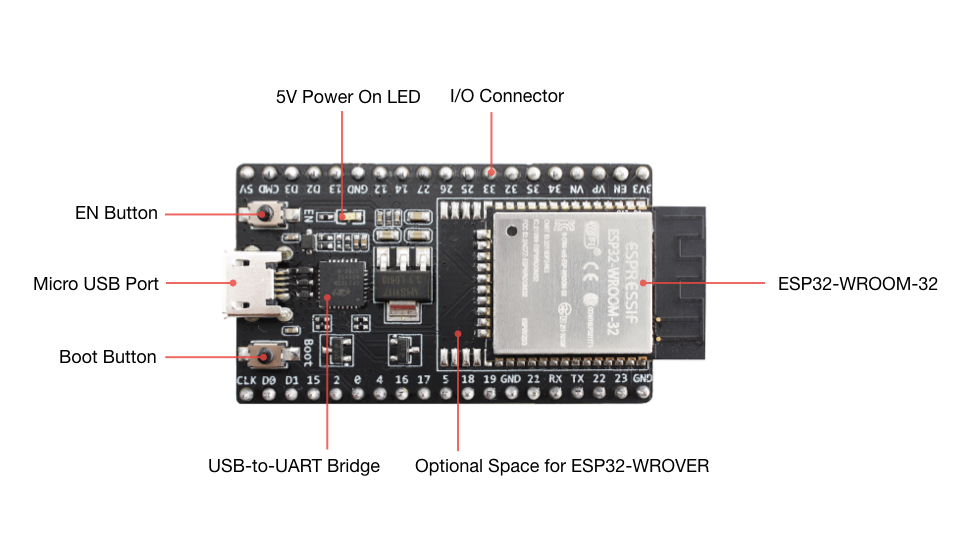
\includegraphics[width=10cm]{imagens/esp32-devkitc-v4-functional-overview.jpg}
    \caption*{Fonte:\cite{ESP32-DevKitCOverview}.}
 \label{esp32DevkitC}
\end{figure}

\begin{figure}[H]
    \centering
    \caption{Pinagem do Microcontrolador ESP32-DevKit C.}
    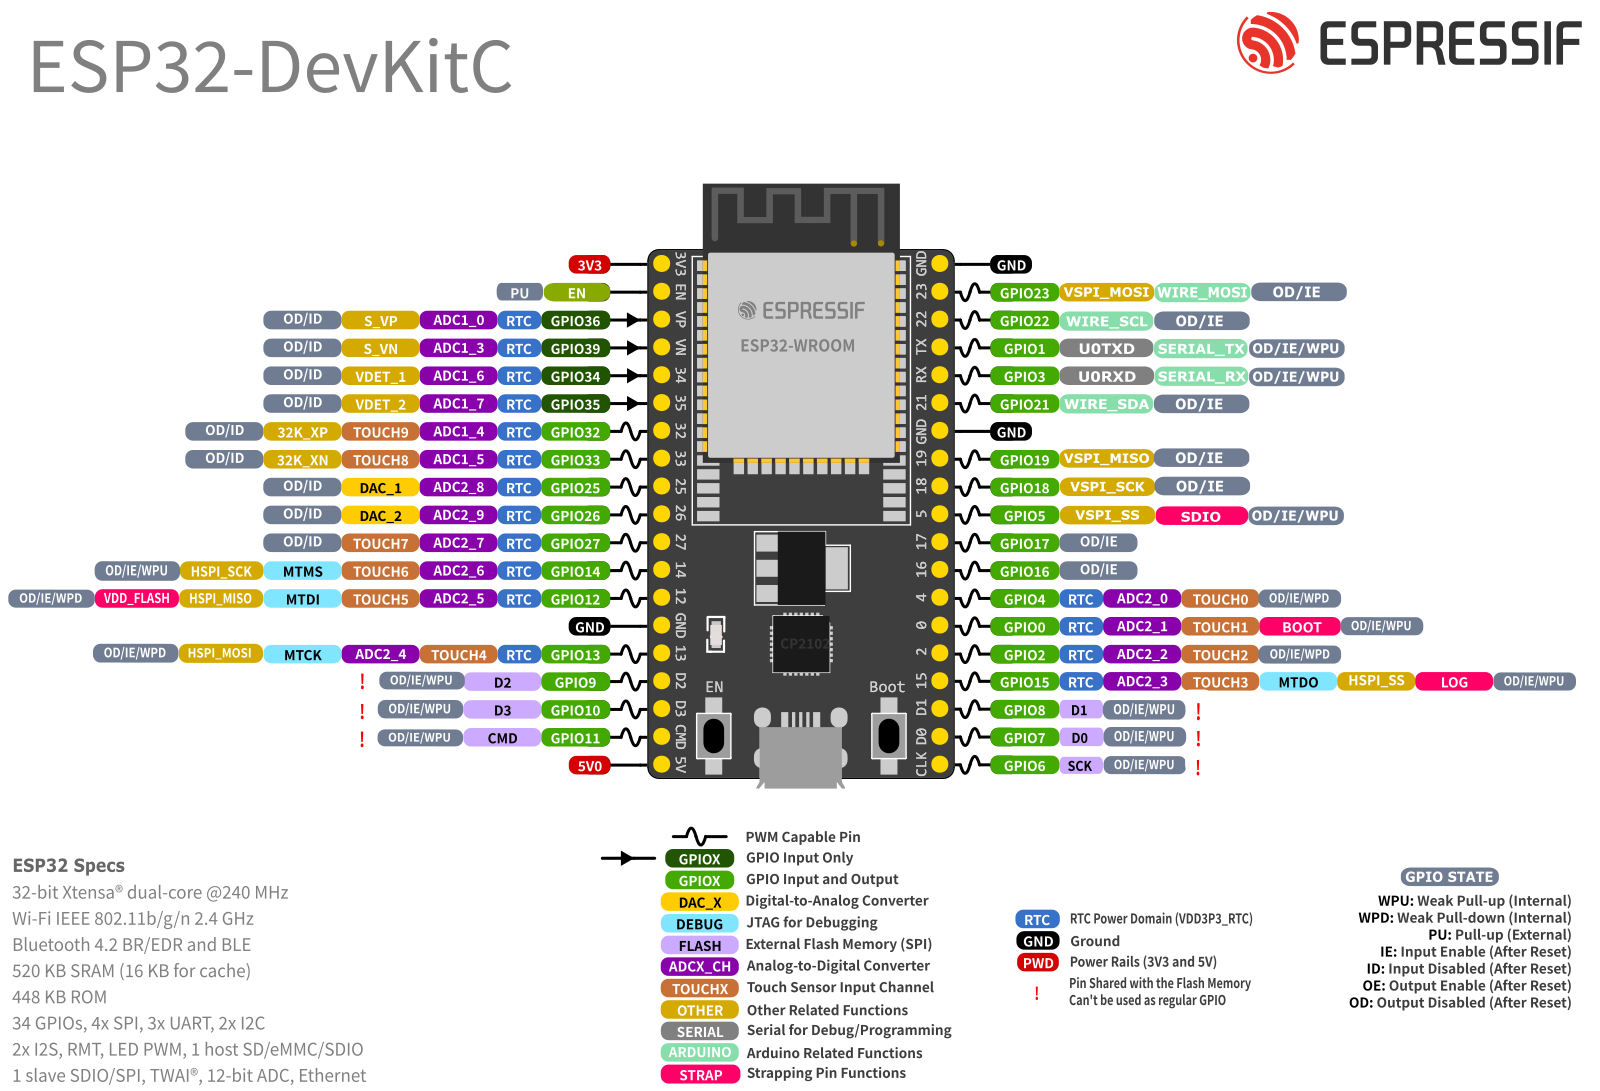
\includegraphics[width=16cm]{imagens/esp32_devkitC_v4_pinlayout.png}
    \caption*{Fonte:\cite{ESP32-DevKitCOverview}.}
 \label{esp32DevkitCPinLayout}
\end{figure}

Apesar dessas vantagens, os níveis lógicos de $3,3V$ exigiram o uso dos drivers IR2110 mencionados anteriormente para a interface com a potência.

\subsection{Lógica de Comutação de Seis Passos}
A lógica de chaveamento constitui o núcleo funcional do ESC. Nesta abordagem, utiliza-se a comutação de seis passos em malha aberta (\textit{Sensorless}). A ponte inversora trifásica é acionada de forma que apenas dois MOSFETs conduzam simultaneamente a cada passo, criando um campo magnético giratório que avança em incrementos de $60^{\circ}$.

\begin{table}[H]
    \centering
    \caption{Sequência de Comutação de Seis Passos e Estado dos MOSFETs}
    \label{tab:logica_seis_passos}
    \begin{tabular}{@{}cccccccc@{}} 
        \toprule
        \textbf{Passo} & \textbf{Pos. Elétrica} & \textbf{High A} & \textbf{Low B} & \textbf{High C} & \textbf{Low A} & \textbf{High B} & \textbf{Low C} \\ \midrule
        1 & 0° -- 60°   & ON & ON  & OFF & OFF & OFF & OFF \\
        2 & 60° -- 120°  & ON & OFF & OFF & OFF & OFF & ON  \\
        3 & 120° -- 180° & OFF& OFF & ON  & OFF & ON  & OFF \\
        4 & 180° -- 240° & OFF& OFF & ON  & ON  & OFF & OFF \\
        5 & 240° -- 300° & OFF& ON  & OFF & ON  & OFF & OFF \\
        6 & 300° -- 360° & OFF& OFF & OFF & OFF & ON  & ON  \\ \bottomrule
    \end{tabular}
    \caption*{Fonte: Elaborado pelo autor.}
\end{table}

\subsection{Implementação Prática com o Periférico MCPWM}
A implementação da comutação no firmware utiliza o periférico dedicado \textit{Motor Control Pulse Width Modulator} (MCPWM) do ESP32 \cite{esp32-technical-reference-manual}. Este módulo desonera a CPU da geração de sinais e insere automaticamente o tempo morto (\textit{Dead Time}) necessário para evitar curto-circuitos na ponte H (shoot-through).

A configuração segue o mapeamento da Tabela \ref{tab:mcpwm_map}, onde o \textit{Duty Cycle} é aplicado ao transistor do lado alto (High-Side) para controle de corrente, enquanto o lado baixo (Low-Side) é mantido em condução plena ou chaveado de forma complementar, dependendo da estratégia de frenagem regenerativa desejada.

\begin{table}[H]
    \centering
    \caption{Mapeamento dos Estados de Comutação para os Geradores MCPWM do ESP32}
    \label{tab:mcpwm_map}
    \resizebox{\textwidth}{!}{%
        \begin{tabular}{@{}ccccccc@{}}
            \toprule
            \textbf{Passo} & \textbf{Fases Energizadas} & \textbf{High-Side} & \textbf{Low-Side} & \textbf{OPR 0 (A)} & \textbf{OPR 1 (B)} & \textbf{OPR 2 (C)} \\ \midrule
            1 & A+ B- & T1 & T4 & PWM / LOW & LOW / ACTIVE & Hi-Z / Hi-Z \\
            2 & A+ C- & T1 & T6 & PWM / LOW & Hi-Z / Hi-Z & LOW / ACTIVE \\
            3 & B+ C- & T3 & T6 & Hi-Z / Hi-Z & PWM / LOW & LOW / ACTIVE \\
            4 & B+ A- & T3 & T2 & LOW / ACTIVE & PWM / LOW & Hi-Z / Hi-Z \\
            5 & C+ A- & T5 & T2 & LOW / ACTIVE & Hi-Z / Hi-Z & PWM / LOW \\
            6 & C+ B- & T5 & T4 & Hi-Z / Hi-Z & LOW / ACTIVE & PWM / LOW \\ \bottomrule
        \end{tabular}
    }
    \flushleft
    \footnotesize{\textit{Nota:} "PWM / LOW" indica modulação. "LOW / ACTIVE" indica condução ao terra. "Hi-Z" alta impedância.} 
\end{table}

\subsection{Estratégia de Partida e Transição para Malha Fechada}

A técnica de detecção de cruzamento por zero da FCEM possui uma limitação física intrínseca: a amplitude da FCEM é proporcional à velocidade do rotor ($e = K_e \cdot \omega$). Na partida ($t=0$), a FCEM é nula, impossibilitando a determinação da posição do rotor pelos comparadores. Para contornar isso, implementou-se uma máquina de estados finitos composta por três estágios:

\begin{enumerate}
    \item \textbf{Alinhamento (Estágio Estático):} 
    Aplica-se uma tensão constante em um par de fases específico (ex: Fase A em High, Fase B em Low) por um período fixo de $500ms$. Isso força o rotor a se alinhar fisicamente com o campo magnético do estator, estabelecendo uma posição inicial conhecida ($\theta_0$) antes do início do movimento.
    
    \item \textbf{Aceleração em Malha Aberta (Blind Commutation):} 
    A partir da posição conhecida, o controlador inicia a sequência de comutação de seis passos utilizando um temporizador interno, ignorando os sinais dos comparadores. A frequência de comutação é incrementada linearmente (Rampa) para acelerar o motor.
    
    Este estágio é mantido pelo menor tempo possível, apenas o suficiente para que o motor atinja cerca de 5\% a 10\% da sua velocidade nominal, ponto em que a amplitude da FCEM supera o limiar de histerese e ruído dos comparadores LM339.
    
    \item \textbf{Transição e Auto-Comutação (Closed-Loop):} 
    Assim que o microcontrolador detecta uma sequência válida de cruzamentos por zero (ZCD) nos comparadores, o sistema realiza o \textit{handover}. O temporizador de malha aberta é desativado e o controle passa a ser orientado a eventos: cada detecção de ZCD dispara uma interrupção que, após um atraso calculado de $30^\circ$ elétricos, executa a próxima comutação de fase. A partir deste momento, o motor opera em malha fechada, auto-sincronizado.
\end{enumerate}

Essa abordagem híbrida elimina a necessidade de rampas longas e ineficientes, garantindo uma partida robusta e uma operação contínua otimizada.


\section{Sistema de Realimentação e Detecção de Cruzamento por Zero}

Para viabilizar a operação em malha fechada sem o uso de sensores de posição dedicados (sensores Hall), implementou-se a técnica de detecção de cruzamento por zero (\textit{Zero-Crossing Detection} - ZCD) da força contraeletromotriz (FCEM). Esta técnica baseia-se no monitoramento da tensão na fase não energizada do motor durante a sequência de comutação de seis passos. O instante em que a FCEM cruza o nível de tensão do ponto neutro do motor indica uma posição angular conhecida do rotor, permitindo a sincronização precisa da comutação eletrônica.

Como o motor utilizado (Turnigy XK3674) possui fechamento interno em triângulo ou estrela sem acesso ao ponto neutro, o sistema de realimentação foi projetado em três estágios: reconstrução do neutro virtual, condicionamento de sinal e comparação.

\subsection{Reconstrução do Neutro Virtual e Divisores de Tensão}

A ausência de um terminal de neutro físico acessível exigiu a criação de um ponto de neutro virtual. Para isso, conectou-se um resistor de $33k\Omega$ em cada uma das três fases do motor ($A, B, C$), unindo as extremidades opostas em um nó comum. Este nó fornece a referência de tensão média do sistema ($V_{ref}$) para os comparadores, conforme topologia clássica para controle trapezoidal \textit{sensorless} \cite{ti2013sensorless}.

Considerando a escalabilidade do projeto para operar com baterias de até 6 células (6S, $\approx 25,2V$), a rede de divisores resistivos foi dimensionada para garantir a segurança do microcontrolador no pior caso de tensão. Utilizou-se uma topologia composta por um resistor de lado alto ($R_{high}$) de $33k\Omega$ e um resistor de lado baixo ($R_{low}$) de $3,3k\Omega$, resultando em um fator de atenuação $\alpha$:

\begin{equation}
    V_{out} = V_{in} \cdot \frac{R_{low}}{R_{high} + R_{low}} = 25,2 \cdot \frac{3,3k}{33k + 3,3k} \approx 2,29V
\end{equation}

Esta configuração garante que a tensão máxima no pino do microcontrolador permaneça abaixo de $3,3V$, preservando uma margem de segurança para picos indutivos (spikes) típicos de comutação.

\subsection{Filtragem de Ruído PWM}

O sinal de tensão proveniente das fases contém componentes de alta frequência resultantes da modulação por largura de pulso (PWM), tipicamente na ordem de $20kHz$. Para evitar múltiplos disparos falsos no comparador, adicionou-se um capacitor cerâmico ($C_f$) de $10nF$ em paralelo com o resistor $R_{low}$, formando um filtro passa-baixa passivo de primeira ordem. A frequência de corte ($f_c$) foi dimensionada para preservar a componente fundamental da FCEM (proporcional à velocidade do motor) enquanto atenua o ruído de chaveamento:

\begin{equation}
    f_c = \frac{1}{2\pi \cdot (R_{high} || R_{low}) \cdot C_f} \approx \frac{1}{2\pi \cdot 3000 \cdot 10 \cdot 10^{-9}} \approx 5,3kHz
\end{equation}

\subsection{Análise e Compensação do Atraso de Fase do Filtro}

A introdução do capacitor $C_f$ no circuito divisor de tensão, embora essencial para a integridade do sinal, insere um polo no sistema que causa um atraso de fase ($\phi$) dependente da frequência. Em um filtro RC de primeira ordem, o atraso de fase entre o sinal de entrada (BEMF real) e o sinal de saída (lido pelo comparador) é dado por \cite{ti2013sensorless}:

\begin{equation}
    \phi = \arctan(2\pi f_{el} R_{eq} C_f) = \arctan\left(\frac{f_{el}}{f_c}\right)
    \label{eq:phase_lag}
\end{equation}

\noindent onde $f_{el}$ é a frequência elétrica fundamental do motor e $f_c$ é a frequência de corte do filtro ($\approx 5,3kHz$).

Este atraso angular é crítico para o sincronismo da comutação. Na estratégia \textit{sensorless} ideal, a comutação das fases deve ocorrer $30^{\circ}$ elétricos após o cruzamento por zero da BEMF. No entanto, devido ao filtro, o comparador detecta o evento de cruzamento com um atraso de $\phi$ graus. Se o microcontrolador aguardar os $30^{\circ}$ teóricos após essa detecção tardia, a comutação efetiva ocorrerá em $30^{\circ} + \phi$, resultando em uma aplicação de torque fora do ponto de máxima eficiência.

Considerando as especificações do motor Turnigy XK3674 ($2200KV$, 4 polos) operando à tensão nominal de $22,2V$, a velocidade máxima teórica aproxima-se de $48.840$ RPM. A frequência elétrica máxima correspondente é:

\begin{equation}
    f_{el\_max} = \frac{RPM \cdot P}{120} = \frac{48840 \cdot 4}{120} \approx 1.628 \text{ Hz}
\end{equation}

Substituindo na Equação \ref{eq:phase_lag}:

\begin{equation}
    \phi_{max} = \arctan\left(\frac{1628}{5300}\right) \approx 17,07^{\circ}
\end{equation}

Como o atraso máximo projetado ($17,07^{\circ}$) é inferior ao intervalo de comutação padrão ($30^{\circ}$), é possível realizar a compensação via software. A estratégia adotada, alinhada às recomendações da literatura especializada \cite{ti2013sensorless}, consiste em calcular dinamicamente o ângulo de atraso $\phi$ a cada ciclo e ajustar o temporizador de espera ($T_{wait}$):

\begin{equation}
    T_{wait} = T_{30^{\circ}} - T_{lag}
\end{equation}

\noindent Onde $T_{30^{\circ}}$ é o período correspondente a $30^{\circ}$ na velocidade atual e $T_{lag}$ é o tempo equivalente ao atraso de fase do filtro. Essa correção assegura que, mesmo em altas rotações, o alinhamento entre os campos do estator e rotor permaneça ortogonal.

\subsection{Estágio Comparador com LM339}

A digitalização dos sinais analógicos é realizada pelo circuito integrado \textbf{LM339N} (encapsulamento DIP-14), que contém quatro comparadores de tensão independentes. A escolha deste componente justifica-se por sua saída em coletor aberto (\textit{Open-Collector}) \cite{tiLM339}. Esta característica permite que o comparador seja alimentado com uma tensão superior (ex: $5V$ ou $12V$) para garantir a linearidade, enquanto a saída é referenciada ao nível lógico do microcontrolador ($3,3V$) através de resistores de \textit{pull-up} de $10k\Omega$.

O circuito utiliza três comparadores configurados da seguinte forma:
\begin{itemize}
    \item \textbf{Entrada Não-Inversora (+):} Tensão da Fase ($A, B$ ou $C$) atenuada e filtrada.
    \item \textbf{Entrada Inversora (-):} Tensão do Neutro Virtual atenuada.
    \item \textbf{Saída:} Conectada a pinos GPIO do ESP32 configurados para interrupção externa.
\end{itemize}

\subsection{Considerações de Sensibilidade e Escalabilidade}

O dimensionamento dos divisores de tensão impõe um compromisso de engenharia (\textit{trade-off}) entre a proteção contra sobretensão e a sensibilidade em baixas velocidades. Com a atenuação de aproximadamente 11:1, sistemas operando com tensões de barramento menores (ex: baterias 2S ou 3S) ou motores em baixa rotação apresentarão sinais de amplitude reduzida na entrada do comparador.

Para mitigar o risco de instabilidade com sinais pequenos, recomenda-se a implementação de \textbf{histerese} no circuito comparador. Isso pode ser realizado através da realimentação positiva, conectando um resistor de alta impedância (ex: $1M\Omega$) entre a saída do comparador e sua entrada não-inversora.

Ressalta-se que a escalabilidade é limitada por dois fatores físicos:
\begin{enumerate}
    \item \textbf{Limite Inferior (3S):} A tensão mínima de operação é definida pelos drivers de gate (IR2110) e pela tensão de limiar ($V_{GS}$) dos MOSFETs. Operar abaixo de $11,1V$ (3S) sem conversores Boost adicionais coloca os transistores na região linear, causando superaquecimento.
    \item \textbf{Limite Superior (6S):} A tensão máxima é estritamente limitada pela tensão de ruptura ($V_{DSS}$) dos MOSFETs utilizados (IRFS7530, $60V$). Embora baterias 7S ($29,4V$) ou 8S ($33,6V$) pareçam estar dentro do limite estático, os picos indutivos gerados durante a comutação podem atingir o dobro da tensão de barramento, excedendo o $V_{DSS}$ e causando falha catastrófica. Portanto, o limite de 6S ($25,2V$) garante a margem de segurança necessária para a robustez do inversor.
\end{enumerate}

\section{Simulação Computacional}
Para validar a lógica de controle e a integridade dos sinais de disparo antes da montagem física, utiliza-se a simulação computacional. Devido à complexidade dos modelos SPICE proprietários para os drivers de gate, opta-se pelo uso de modelos comportamentais equivalentes em software de simulação de circuitos (ex: LTSpice ou Proteus). A simulação foca na verificação das formas de onda de tensão de linha e de fase, bem como na garantia de que a sequência de seis passos não gera sobreposição de condução nos braços do inversor.

\section{Montagem e Prototipagem}
A etapa final consiste na integração física dos subsistemas. O controlador é montado em uma placa de circuito impresso (PCB) desenhada para suportar as altas correntes do barramento DC, com trilhas reforçadas e planos de terra adequados. O microcontrolador é programado com a lógica desenvolvida e o sistema é submetido a testes de bancada, iniciando com cargas leves e alimentação limitada para verificação de segurança (teste de fumaça), progredindo para o acionamento do motor em rampa de velocidade para validação do protótipo funcional.

Todas as etapas de validação e os resultados obtidos, tanto na simulação quanto nos ensaios práticos, são documentados no capítulo subsequente de Resultados.

